Para experimentar, utilizamos una computadora con las siguientes características:

\begin{itemize}
 \item Procesador: 
 \item RAM: 
\end{itemize}

La primer etapa de experimentación consistió en verificar empíricamente la cota de complejidad temporal obtenida teóricamente para el algoritmo completo. Estas primeras dos figuras nos permiten ver que efectivamente nuestro algoritmo es $O(n * log(n))$

\begin{figure}[H]
    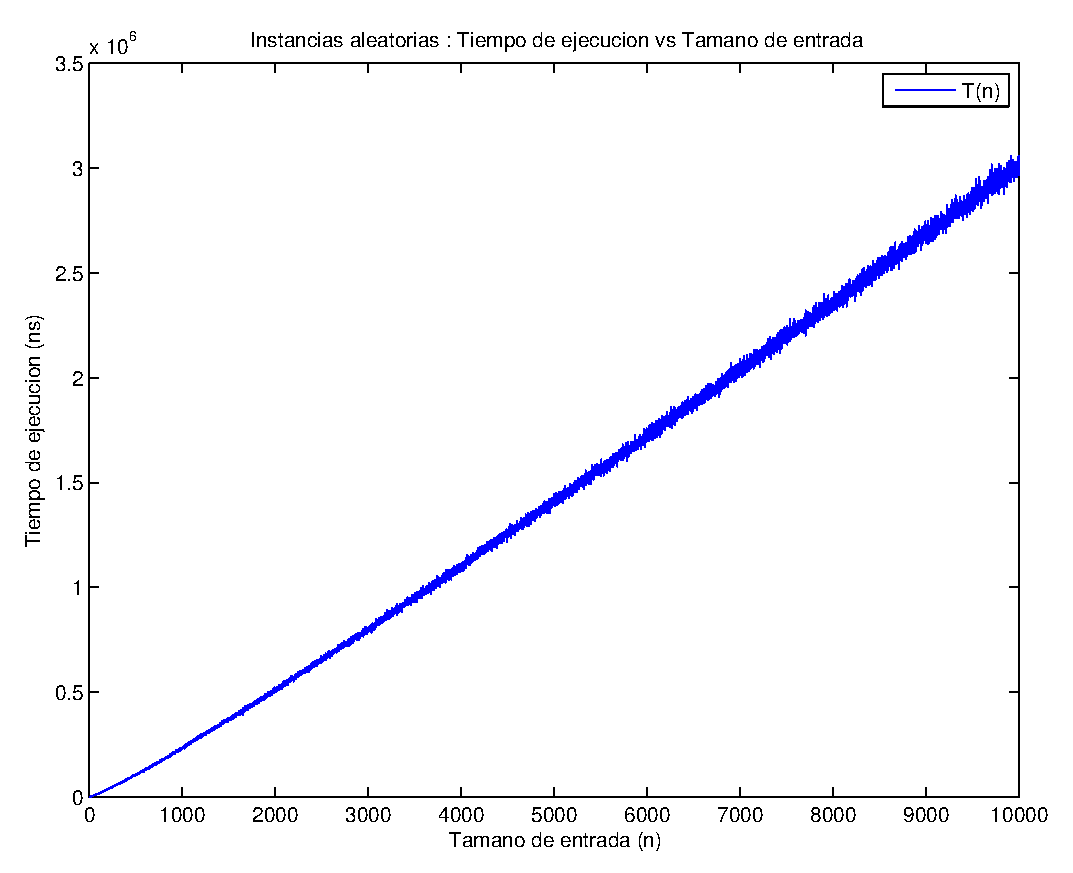
\includegraphics[width=0.5\linewidth]{problema1/graficos/problema1_aleatoria_10000.eps}
    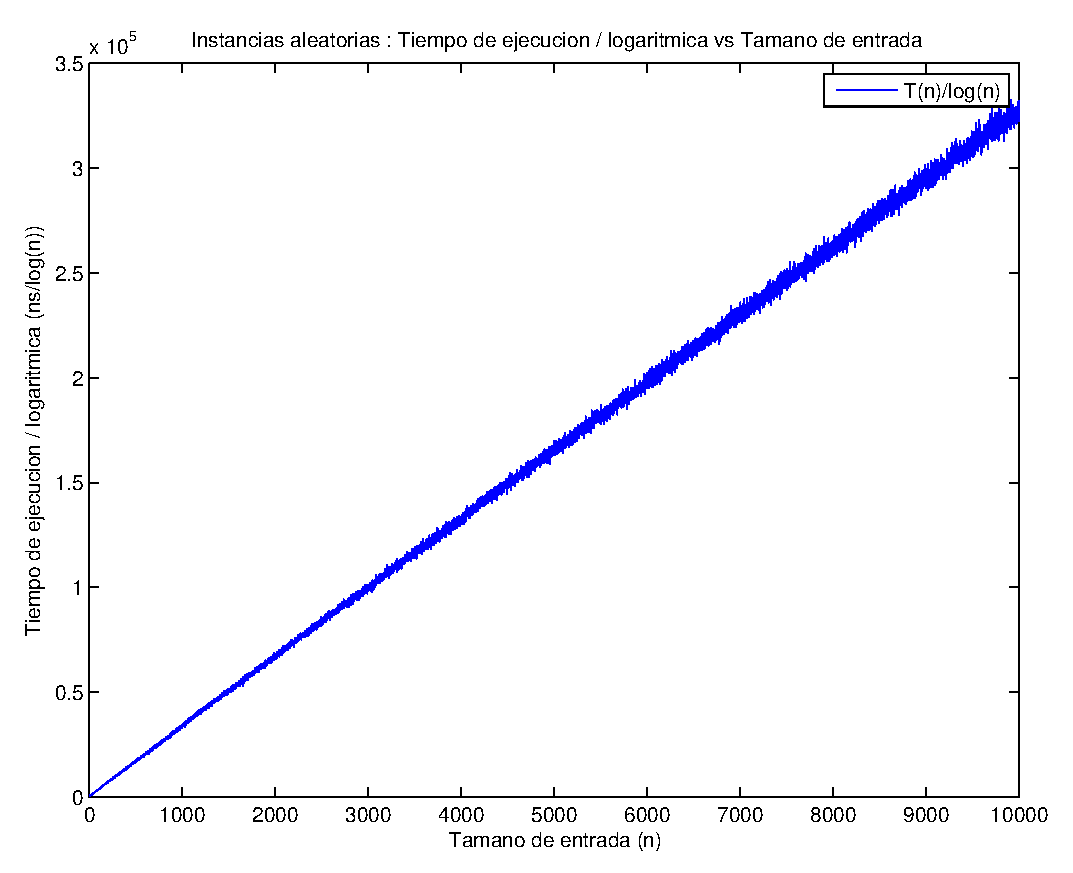
\includegraphics[width=0.5\linewidth]{problema1/graficos/problema1_aleatoria_10000_div_logn.eps}
\end{figure}
\emph{\hspace{2,5cm}Figura 1: n <= 10000 \hspace{3cm}Figura 2: Idem, pero dividido por $log(n)$}

Como se puede observar en la figura 2, una vez que dividimos por $log n$ a cada resultado obtenido por nuestras mediciones, éstos forman una recta. Es decir, $T(n)/log(n) \in O(n)$. Esto significa que la complejidad del algoritmo en su totalidad es de $O(n * log(n))$.

Según nuestro análisis, la complejidad temporal de la solución es dominada por la etapa de ordenamiento. Dado que el algoritmo utilizado para este fin pertenece a librerías estándares de C++, la experimentación subsiguiente se realizó sobre instancias donde la lista de entrada se encuentra ordenada, eliminando la etapa de ordenamiento. Esto permitió constatar si el ciclo final incurre efectivamente en un costo a lo sumo lineal, y poder medir el impacto de la ordenamiento en la complejidad temporal final.

En las figuras siguientes podemos observar que, sin contar la etapa de ordenamiento, efectivamente nuestro algoritmo es $O(n)$. Para lograr esto, simplemente utilizamos entradas en las cuales los camiones estén ordenados, y por esto no haga falta realizar el sorting. Para hacer el gráfico mas interesante, comparamos casos donde todos los camiones llegan en días distintos contra casos donde actualiza seguido cuál es el día óptimo.

  \begin{figure}[H]
    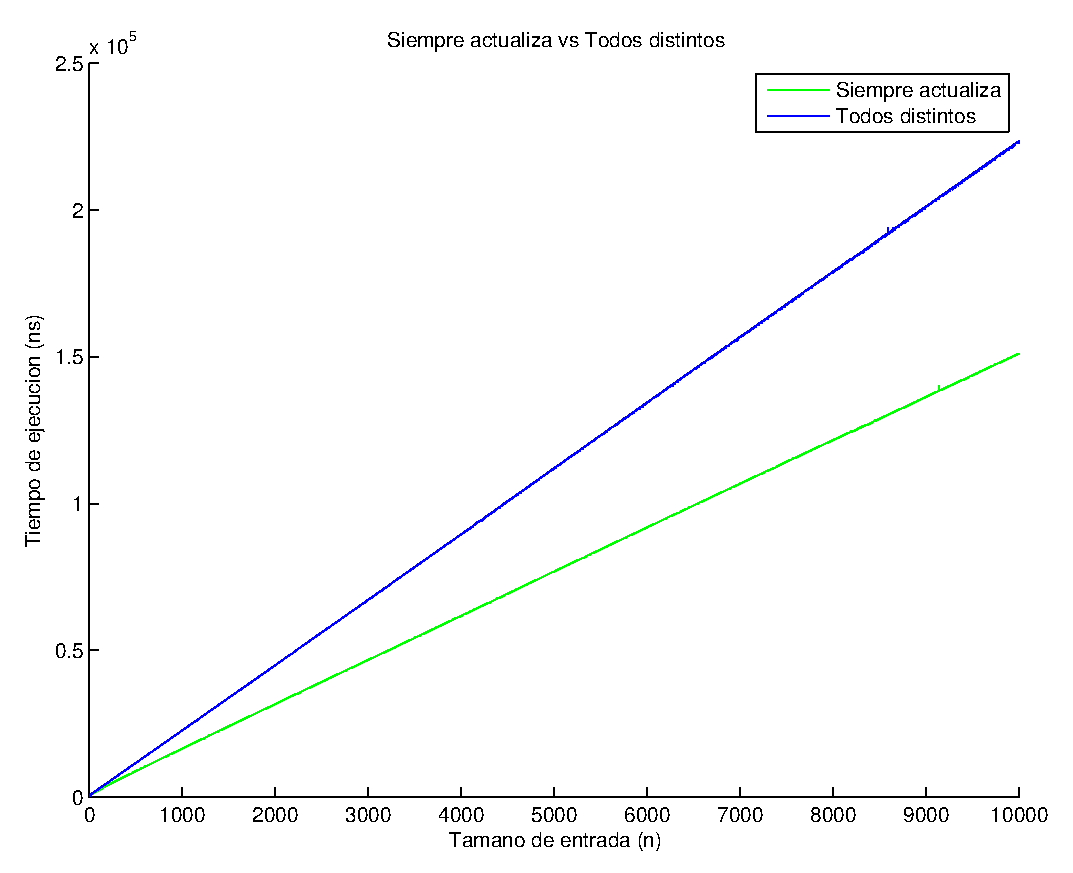
\includegraphics[width=0.5\linewidth]{problema1/graficos/problema1_ordenada_siempre_actualiza_10000_vs_problema1_ordenada_todos_distintos_10000.eps}
    %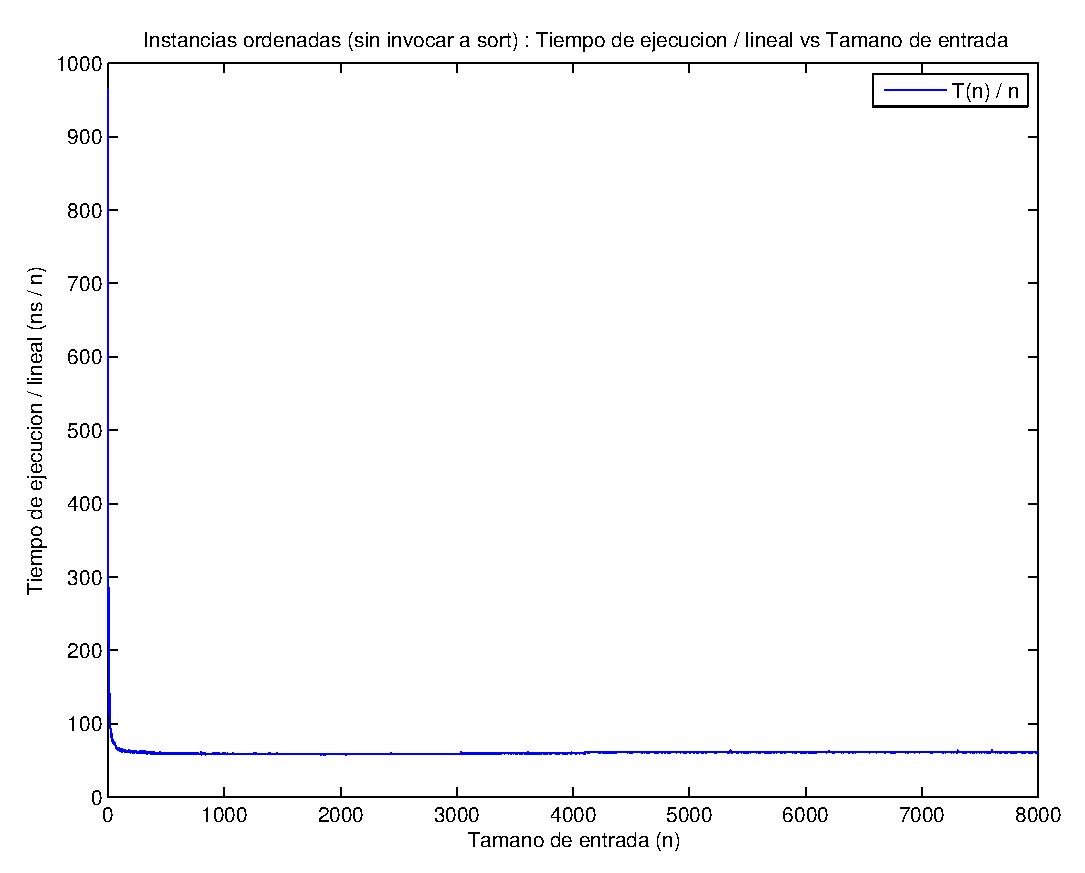
\includegraphics[width=0.5\linewidth]{problema2/graficos/problema2_ordenada_8000_div_n.eps}
\end{figure}
\emph{\hspace{2,5cm}Figura 3: n <= 10000 \hspace{3cm}Figura 4: ACA PONEMOS ALGO???}

Curiosamente, ``siempre actualiza'' es mejor que ``Todos distintos''. Investigamos y llegamos a la conclusión que esto se debe a como creamos las instancias de entrada. Las creamos siguiendo la siguiente secuencia:

\begin{verbatim}
  1,2,2,3,3,3,4,4,4,4 ...
\end{verbatim}

Como tiene números repetidos, el algoritmo saltea varias iteraciones en la parte del siguiente \emph{for}.

\begin{verbatim}
  for (; (j < e.cant_dias) && (dias[j] - dias[i] < e.cant_dias_inspeccion); ++j)
      ;
\end{verbatim}

Por esta razón, termina siendo mejor que el de ``Todos distintos''.
